%%% For single-sided printing
%\documentclass[11pt,a4paper]{report}
%\usepackage[top=25mm,bottom=25mm,right=25mm,left=30mm,head=12.5mm,foot=12.5mm]{geometry}
%\let\openright=\clearpage

%%% For two-sided printing:
\documentclass[11pt,a4paper,twoside,openright]{report}
\usepackage[top=25mm,bottom=25mm,right=25mm,left=30mm,head=12.5mm,foot=12.5mm]{geometry}
\usepackage[font={small,it}]{caption}
\let\openright=\cleardoublepage

%%% References
\usepackage{dirtree}
\usepackage{hyperref}
\usepackage{nameref}
\usepackage[
  atend,
  numbered
]{bookmark}

%% Description reference labels
\makeatletter
\newcommand{\numbersections}{\renewcommand{\Hy@numberline}[1]{##1. }}
\newcommand{\nonumbersections}{\renewcommand{\Hy@numberline}[1]{}}
\def\namedlabel#1#2{\begingroup
    #2%
    \def\@currentlabel{#2}%
    \phantomsection\label{#1}\endgroup
}
\makeatother

%%% Charts
\usepackage{pgf-pie}
\usepackage{pgfplots}

%%% Footnotes
\usepackage{footnote}
\makesavenoteenv{tabular}

%%% Definition of useful macros
%%% Tento soubor obsahuje definice různých užitečných maker a prostředí %%%
%%% Další makra připisujte sem, ať nepřekáží v ostatních souborech.     %%%

\usepackage[a-2u]{pdfx}     % výsledné PDF bude ve standardu PDF/A-2u

\usepackage{ifpdf}
\usepackage{ifxetex}
\usepackage{ifluatex}
\usepackage{float}
\usepackage{tikz}
\usetikzlibrary{shapes.geometric,shapes.arrows,decorations.pathmorphing}
\usetikzlibrary{matrix,chains,scopes,positioning,arrows,fit}

\nocite{*}
%%% Nastavení pro použití samostatné bibliografické databáze.
\usepackage[
   backend=bibtex
%  ,style=iso-authoryear
  ,style=iso-numeric
  ,sortlocale=cs_CZ
  ,alldates=iso
  ,bibencoding=UTF8
  %,block=ragged
]{biblatex}
\let\cite\parencite
\bibliography{literatura}

%% Přepneme na českou sazbu, fonty Latin Modern a kódování češtiny
\ifthenelse{\boolean{xetex}\OR\boolean{luatex}}
   { % use fontspec and OpenType fonts with utf8 engines
			\usepackage[english,slovak,czech]{babel}
			\usepackage[autostyle,english=british,czech=quotes]{csquotes}
			\usepackage{fontspec}
			\defaultfontfeatures{Ligatures=TeX,Scale=MatchLowercase}
   }
   {
			\usepackage[english,slovak,czech]{babel}
			\usepackage{lmodern}
			\usepackage[T1]{fontenc}
			\usepackage{textcomp}
			\usepackage[utf8]{inputenc}
			\usepackage[autostyle,english=british,czech=quotes]{csquotes}
	 }
\ifluatex
\makeatletter
\let\pdfstrcmp\pdf@strcmp
\makeatother
\fi

%%% Další užitečné balíčky (jsou součástí běžných distribucí LaTeXu)
\usepackage{amsmath}        % rozšíření pro sazbu matematiky
\usepackage{amsfonts}       % matematické fonty
\usepackage{amssymb}        % symboly
\usepackage{amsthm}         % sazba vět, definic apod.
\usepackage{bm}             % tučné symboly (příkaz \bm)
\usepackage{graphicx}       % vkládání obrázků
\usepackage{listings}       % vylepšené prostředí pro strojové písmo
\usepackage{fancyhdr}       % prostředí pohodlnější nastavení hlavy a paty stránek
\usepackage{icomma}         % inteligetní čárka v matematickém módu
\usepackage{dcolumn}        % lepší zarovnání sloupců v tabulkách
\usepackage{booktabs}       % lepší vodorovné linky v tabulkách
\usepackage{listings}       % Code formatting
\usepackage{color}       % Code formatting


\definecolor{red}{rgb}{0.6,0,0} % for strings
\definecolor{blue}{rgb}{0,0,0.6}
\definecolor{green}{rgb}{0,0.8,0}
\definecolor{cyan}{rgb}{0.0,0.6,0.6}

\lstset{
language=csh,
basicstyle=\footnotesize\ttfamily,
numbers=left,
numberstyle=\tiny,
numbersep=5pt,
tabsize=2,
extendedchars=true,
breaklines=true,
frame=b,
stringstyle=\color{blue}\ttfamily,
showspaces=false,
showtabs=false,
xleftmargin=17pt,
framexleftmargin=17pt,
framexrightmargin=5pt,
framexbottommargin=4pt,
showstringspaces=false,
}

\usepackage{caption}
% \DeclareCaptionFont{white}{\color{white}}
% \DeclareCaptionFormat{listing}{\colorbox{blue}{\parbox{\textwidth}{\hspace{15pt}#1#2#3}}}
% \captionsetup[lstlisting]{format=listing,labelfont=white,textfont=white, singlelinecheck=false, margin=0pt, font={bf,footnotesize}}

\makeatletter
\@ifpackageloaded{xcolor}{
   \@ifpackagewith{xcolor}{usenames}{}{\PassOptionsToPackage{usenames}{xcolor}}
  }{\usepackage[usenames]{xcolor}} % barevná sazba
\makeatother
\usepackage{multicol}       % práce s více sloupci na stránce
\usepackage{enumitem}
\setlist[itemize]{noitemsep, topsep=0pt, partopsep=0pt}
\setlist[enumerate]{noitemsep, topsep=0pt, partopsep=0pt}
\setlist[description]{noitemsep, topsep=0pt, partopsep=0pt}

\usepackage{tocloft}
\setlength\cftparskip{0pt}
\setlength\cftbeforechapskip{1.5ex}
\setlength\cftfigindent{0pt}
\setlength\cfttabindent{0pt}
\setlength\cftbeforeloftitleskip{0pt}
\setlength\cftbeforelottitleskip{0pt}
\setlength\cftbeforetoctitleskip{0pt}
\renewcommand{\cftlottitlefont}{\Huge\bfseries\sffamily}
\renewcommand{\cftloftitlefont}{\Huge\bfseries\sffamily}
\renewcommand{\cfttoctitlefont}{\Huge\bfseries\sffamily}

% vyznaceni odstavcu
\parindent=0pt
\parskip=11pt

% zakaz vdov a sirotku - jednoradkovych pocatku ci koncu odstavcu na prechodu mezi strankami
\clubpenalty=1000
\widowpenalty=1000
\displaywidowpenalty=1000

% nastaveni radkovani
\renewcommand{\baselinestretch}{1.20}

% nastaveni pro nadpisy - tucne a bezpatkove
\usepackage{sectsty}    
\allsectionsfont{\sffamily}

% nastavení hlavy a paty stránek
\fancyhf{}
\fancyhead[RO,LE]{\rightmark}
\fancyfoot[RO,LE]{\thepage}
\renewcommand{\footrulewidth}{.5pt}
\fancypagestyle{plain}{%
\fancyhf{} % clear all header and footer fields
\fancyfoot[RO,LE]{\thepage}
\renewcommand{\headrulewidth}{0pt}
\renewcommand{\footrulewidth}{0.5pt}}

% Tato makra přesvědčují mírně ošklivým trikem LaTeX, aby hlavičky kapitol
% sázel příčetněji a nevynechával nad nimi spoustu místa. Směle ignorujte.
\makeatletter
\def\@makechapterhead#1{
  {\parindent \z@ \raggedright \sffamily
   \Huge\bfseries \thechapter. #1
   \par\nobreak
   \vskip 20\p@
}}
\def\@makeschapterhead#1{
  {\parindent \z@ \raggedright \sffamily
   \Huge\bfseries #1
   \par\nobreak
   \vskip 20\p@
}}
\makeatother

% Trochu volnější nastavení dělení slov, než je default.
\lefthyphenmin=2
\righthyphenmin=2

% Zapne černé "slimáky" na koncích řádků, které přetekly, abychom si
% jich lépe všimli.
\overfullrule=1mm

%% Balíček hyperref, kterým jdou vyrábět klikací odkazy v PDF,
%% ale hlavně ho používáme k uložení metadat do PDF (včetně obsahu).
%% Většinu nastavítek přednastaví balíček pdfx.
\hypersetup{unicode}
\hypersetup{breaklinks=true}
\hypersetup{hidelinks}

%%% Prostředí pro sazbu kódu, případně vstupu/výstupu počítačových
%%% programů. (Vyžaduje balíček listings -- fancy verbatim.)
\lstnewenvironment{code}{\lstset{basicstyle=\small, frame=single}}{}





%%% DEFINICE ZÁKLADNÍCH PROMĚNNÝCH
\def\TypPrace{BP}               % bakalářská práce/bachelor thesis
%\def\TypPrace{DP}              % diplomová práce/master thesis
%\def\Jazyk{cze}                % čeština/czech
%\def\Jazyk{slo}                % slovenština/slovak
\def\Jazyk{eng}                 % angličtina/english

%%% Title of the thesis in the language used in the text (exact according to assignment)
\def\NazevPrace{Development of a documentation generating application for .NET libraries}

%%% Tento soubor obsahuje definice různých užitečných maker a prostředí %%%
%%% Další makra připisujte sem, ať nepřekáží v ostatních souborech.     %%%

\usepackage[a-2u]{pdfx}     % výsledné PDF bude ve standardu PDF/A-2u

\usepackage{ifpdf}
\usepackage{ifxetex}
\usepackage{ifluatex}
\usepackage{float}
\usepackage{tikz}
\usetikzlibrary{shapes.geometric,shapes.arrows,decorations.pathmorphing}
\usetikzlibrary{matrix,chains,scopes,positioning,arrows,fit}

\nocite{*}
%%% Nastavení pro použití samostatné bibliografické databáze.
\usepackage[
   backend=bibtex
%  ,style=iso-authoryear
  ,style=iso-numeric
  ,sortlocale=cs_CZ
  ,alldates=iso
  ,bibencoding=UTF8
  %,block=ragged
]{biblatex}
\let\cite\parencite
\bibliography{literatura}

%% Přepneme na českou sazbu, fonty Latin Modern a kódování češtiny
\ifthenelse{\boolean{xetex}\OR\boolean{luatex}}
   { % use fontspec and OpenType fonts with utf8 engines
			\usepackage[english,slovak,czech]{babel}
			\usepackage[autostyle,english=british,czech=quotes]{csquotes}
			\usepackage{fontspec}
			\defaultfontfeatures{Ligatures=TeX,Scale=MatchLowercase}
   }
   {
			\usepackage[english,slovak,czech]{babel}
			\usepackage{lmodern}
			\usepackage[T1]{fontenc}
			\usepackage{textcomp}
			\usepackage[utf8]{inputenc}
			\usepackage[autostyle,english=british,czech=quotes]{csquotes}
	 }
\ifluatex
\makeatletter
\let\pdfstrcmp\pdf@strcmp
\makeatother
\fi

%%% Další užitečné balíčky (jsou součástí běžných distribucí LaTeXu)
\usepackage{amsmath}        % rozšíření pro sazbu matematiky
\usepackage{amsfonts}       % matematické fonty
\usepackage{amssymb}        % symboly
\usepackage{amsthm}         % sazba vět, definic apod.
\usepackage{bm}             % tučné symboly (příkaz \bm)
\usepackage{graphicx}       % vkládání obrázků
\usepackage{listings}       % vylepšené prostředí pro strojové písmo
\usepackage{fancyhdr}       % prostředí pohodlnější nastavení hlavy a paty stránek
\usepackage{icomma}         % inteligetní čárka v matematickém módu
\usepackage{dcolumn}        % lepší zarovnání sloupců v tabulkách
\usepackage{booktabs}       % lepší vodorovné linky v tabulkách
\usepackage{listings}       % Code formatting
\usepackage{color}       % Code formatting


\definecolor{red}{rgb}{0.6,0,0} % for strings
\definecolor{blue}{rgb}{0,0,0.6}
\definecolor{green}{rgb}{0,0.8,0}
\definecolor{cyan}{rgb}{0.0,0.6,0.6}

\lstset{
language=csh,
basicstyle=\footnotesize\ttfamily,
numbers=left,
numberstyle=\tiny,
numbersep=5pt,
tabsize=2,
extendedchars=true,
breaklines=true,
frame=b,
stringstyle=\color{blue}\ttfamily,
showspaces=false,
showtabs=false,
xleftmargin=17pt,
framexleftmargin=17pt,
framexrightmargin=5pt,
framexbottommargin=4pt,
showstringspaces=false,
}

\usepackage{caption}
% \DeclareCaptionFont{white}{\color{white}}
% \DeclareCaptionFormat{listing}{\colorbox{blue}{\parbox{\textwidth}{\hspace{15pt}#1#2#3}}}
% \captionsetup[lstlisting]{format=listing,labelfont=white,textfont=white, singlelinecheck=false, margin=0pt, font={bf,footnotesize}}

\makeatletter
\@ifpackageloaded{xcolor}{
   \@ifpackagewith{xcolor}{usenames}{}{\PassOptionsToPackage{usenames}{xcolor}}
  }{\usepackage[usenames]{xcolor}} % barevná sazba
\makeatother
\usepackage{multicol}       % práce s více sloupci na stránce
\usepackage{enumitem}
\setlist[itemize]{noitemsep, topsep=0pt, partopsep=0pt}
\setlist[enumerate]{noitemsep, topsep=0pt, partopsep=0pt}
\setlist[description]{noitemsep, topsep=0pt, partopsep=0pt}

\usepackage{tocloft}
\setlength\cftparskip{0pt}
\setlength\cftbeforechapskip{1.5ex}
\setlength\cftfigindent{0pt}
\setlength\cfttabindent{0pt}
\setlength\cftbeforeloftitleskip{0pt}
\setlength\cftbeforelottitleskip{0pt}
\setlength\cftbeforetoctitleskip{0pt}
\renewcommand{\cftlottitlefont}{\Huge\bfseries\sffamily}
\renewcommand{\cftloftitlefont}{\Huge\bfseries\sffamily}
\renewcommand{\cfttoctitlefont}{\Huge\bfseries\sffamily}

% vyznaceni odstavcu
\parindent=0pt
\parskip=11pt

% zakaz vdov a sirotku - jednoradkovych pocatku ci koncu odstavcu na prechodu mezi strankami
\clubpenalty=1000
\widowpenalty=1000
\displaywidowpenalty=1000

% nastaveni radkovani
\renewcommand{\baselinestretch}{1.20}

% nastaveni pro nadpisy - tucne a bezpatkove
\usepackage{sectsty}    
\allsectionsfont{\sffamily}

% nastavení hlavy a paty stránek
\fancyhf{}
\fancyhead[RO,LE]{\rightmark}
\fancyfoot[RO,LE]{\thepage}
\renewcommand{\footrulewidth}{.5pt}
\fancypagestyle{plain}{%
\fancyhf{} % clear all header and footer fields
\fancyfoot[RO,LE]{\thepage}
\renewcommand{\headrulewidth}{0pt}
\renewcommand{\footrulewidth}{0.5pt}}

% Tato makra přesvědčují mírně ošklivým trikem LaTeX, aby hlavičky kapitol
% sázel příčetněji a nevynechával nad nimi spoustu místa. Směle ignorujte.
\makeatletter
\def\@makechapterhead#1{
  {\parindent \z@ \raggedright \sffamily
   \Huge\bfseries \thechapter. #1
   \par\nobreak
   \vskip 20\p@
}}
\def\@makeschapterhead#1{
  {\parindent \z@ \raggedright \sffamily
   \Huge\bfseries #1
   \par\nobreak
   \vskip 20\p@
}}
\makeatother

% Trochu volnější nastavení dělení slov, než je default.
\lefthyphenmin=2
\righthyphenmin=2

% Zapne černé "slimáky" na koncích řádků, které přetekly, abychom si
% jich lépe všimli.
\overfullrule=1mm

%% Balíček hyperref, kterým jdou vyrábět klikací odkazy v PDF,
%% ale hlavně ho používáme k uložení metadat do PDF (včetně obsahu).
%% Většinu nastavítek přednastaví balíček pdfx.
\hypersetup{unicode}
\hypersetup{breaklinks=true}
\hypersetup{hidelinks}

%%% Prostředí pro sazbu kódu, případně vstupu/výstupu počítačových
%%% programů. (Vyžaduje balíček listings -- fancy verbatim.)
\lstnewenvironment{code}{\lstset{basicstyle=\small, frame=single}}{}





%%% Author's name - Firstname and Lastname
\def\AutorPrace{Denis Akopyan}

%%% Year of submission and month (verbally) - month YYYY
\def\DatumOdevzdani{December 2022}

%%% Supervisor: First name and surname with titles
\def\Vedouci{Ing. Jarmila Pavlíčková, Ph.D.}

%%% Consultant: First name and surname with titles
\def\Konzultant{}

%%% Study program
\def\StudijniProgram{Applied Informatics}

%%% Study program - specialization
\def\Specializace{}

%%% Field of study
\def\StudijniObor{Applied Informatics}

%%% Optional thanks (the supervisor, the consultant, the borrower of software, literature, etc)
\def\Podekovani{%
Many thanks to Ing. Jarmila Pavlíčková, Ph.d. for supervising the majority of my thesis.
}

%%% Abstrakt (doporučený rozsah cca 150-250 slov; nejedná se o zadání práce)
\def\Abstrakt{%
Zaměřením dané bakalářské práce je výzkum a vývoj aplikace pro generování programátorské dokumentace .NET knihoven. Hlavním cílem bylo vytvoření nástroje pro .NET vývojáře, kteří chtějí extrahovat dokumentaci zdrojového kódu a exportovat ji do požadovaného výstupu, a zároveň zachovat aplikaci rozšiřitelnou, multiplatformní a uživatelsky přístupnou.\

Teoretická část práce se bude zabývát plánováním vývoje a očekáváným výsledkem projektu.

Empirická část popíše vývoj samotný a zaměřuje se na tvorbu oddělené projektové struktury.

Očekáváným výsledkem bakalářské práce bude funkční, multiplatformní a open-source aplikace, která umožňuje generování dokumentace z .NET knihoven, a zároveň je rozšiřitelná prostřednictvím modulů.
}
\def\AbstraktEN{%
This thesis aims to research and develop a documentation-generating application for .NET libraries.
The main objective was to create a tool for .NET developers that want to extract source code documentation and export it into their desired format while keeping the application extensible, cross-platform, and easy to use.

The theoretical part of the thesis shall cover the development planning and the expected result of the
project.

The empirical part of the thesis illustrates the exact process of development. Designing a decoupled
project structure had the most attention dedicated to it.

The expected result of this thesis project is a working cross-platform and open-source application that can
generate documentation from .NET libraries and is extensible via plugins.
}

%%% 3 až 5 klíčových slov (doporučeno)
\def\KlicovaSlova{vývoj, tvorba, aplikace, generování, dokumentace, dotnet, .NET, knihoven}
\def\KlicovaSlovaEN{development, application, generating, documentation, dotnet, .NET, libraries}

%%% Kody podle klasifikace JEL
\def\JEL{C88, O30}

%%% Fix height
\raggedbottom

%%% Title page and various mandatory information pages
\begin{document}
\include{beginning}

%%% A page with automatically generated content of the thesis
\setcounter{tocdepth}{2}
\tableofcontents

%%% List of figures in the thesis
\openright
\listoffigures

%%% List of tables in the thesis (optionally)
\clearpage
\listoftables
\lstlistoflistings

%%% List of abbreviations and glossary in the thesis (optionally)
\chapter*{List of abbreviations}

\begin{multicols}{2}
    \raggedright
    \begin{description}
        \item [\namedlabel{itm:html}{HTML}] Hypertext Markup Language
        \item [\namedlabel{itm:ux}{UX}] User eXperience
        \item [\namedlabel{itm:ui}{UI}] User Interface
        \item [\namedlabel{itm:gui}{GUI}] Graphical User Interface
        \item [\namedlabel{itm:rtf}{RTF}] Rich Text Format
        \item [\namedlabel{itm:xml}{XML}] eXtended Markup Language
        \item [\namedlabel{itm:cli}{CLI}] Command Line Interface
        \item [\namedlabel{itm:api}{API}] Application Programming Interface
        \item [\namedlabel{itm:pdf}{PDF}] Portable Document Format
        \item [\namedlabel{itm:cicd}{CI/CD}] Continuous integration and continuous deployment
        \item [\namedlabel{itm:os}{OS}] Operating System
        \item [\namedlabel{itm:mvvm}{MVVM}] Model View ViewModel, structural design pattern
        \item [\namedlabel{itm:solid}{SOLID}] Single Responsibility Principle, Open-Closed Principle, Liskov Substitution Principle, Interface Segregation Principle, Dependency Inversion Principle
        \item [\namedlabel{itm:di}{DI}] Dependency Injection
        \item [\namedlabel{itm:wpf}{WPF}] Windows Presentation Framework
        \item [\namedlabel{itm:url}{URL}] Uniform Resource Locator
        \item [\namedlabel{itm:ascii}{ASCII}] American Standard Code for Information Interchange
    \end{description}
\end{multicols}


\chapter*{Glossary}

\begin{description}
    \item [\namedlabel{gloss:dotnetlabel}{.NET}] A free, cross-platform, open-source developer platform for building many different types of applications \cite{microsoft_what_2022}
    \item [\namedlabel{gloss:aspnetcore}{ASP.NET Core}] A cross-platform, high-performance, open-source framework for building modern, cloud-enabled, Internet-connected apps \cite{anderson_overview_2022}
    \item [\namedlabel{gloss:nuget}{NuGet}] Package manager for .NET projects \cite{microsoft_nuget_2022}
    \item [\namedlabel{gloss:git}{Git}] A free and open-source distributed version control system designed to handle everything from small to very large projects with speed and efficiency \cite{git_git_2022}
    \item [\namedlabel{gloss:markdown}{Markdown}] A popular lightweight markup language that is used to add formatting elements to plaintext text documents \cite{cone_getting_2022}
    \item [\namedlabel{gloss:winforms}{Windows Forms}] A.k.a. WinForms, a \ref{itm:gui} framework from Microsoft bundled with .NET \cite{george_what_2022}
    \item [\namedlabel{gloss:asciiart}{ASCII art}] text-based images consisting of \ref{itm:ascii} characters \cite{randal_ascii_2015}
\end{description}

\pagestyle{fancy}
%%% The individual chapters of the thesis are stored in separate files for clarity
\chapter*{Introduction}
\addcontentsline{toc}{chapter}{Introduction}

Source code documentation is an essential part of any quality project. Unfortunately, writing and keeping such documentation up to date is often overlooked or inconvenient for various reasons, such as strict deadlines. That might lead to the degradation of project quality, as developers who leave said projects usually take their know-how with them without properly passing it down to their replacements.

In cases where source code documentation has a higher priority than usual, extracting said documentation from the source code into a searchable, public format such as \ref{itm:html} is good practice. Documentation-generating tools accomplish that. The primary benefit of this practice is the resulting comprehensive overview of the source code, accessible to interested parties.

For Microsoft \ref{gloss:dotnetlabel} projects, there is a selection of documentation-generating tools available, which includes: DocFX, Doxygen, SourceBrowser, and others. These solutions primarily generate output in \ref{itm:html}, which is sufficient for most projects. However, these tools often lack support for output formats like \ref{itm:pdf}, \ref{gloss:markdown}, or custom. Moreover, the customization of these tools is minimal, preventing projects from being able to fit such tools to their exact needs. Furthermore, their \ref{itm:ui}/\ref{itm:ux} leaves much to be desired, introducing an unnecessary learning curve and lowering usability.

With that in mind, there is visible room for improvement. A desirable documentation-generating tool would be easy to use, modern, extensible, rich in output format support, and performant. Satisfying the desires of an modern extensible application requires the thorough use of programming design patterns such as \ref{itm:solid}, \ref{itm:di}, and \ref{itm:mvvm}.

\section*{Motivation}
\addcontentsline{toc}{section}{Motivation}

The motivation for creating a custom tool is primarily a personal need to provide easy access to code documentation. Since most open-source projects are hosted either on GitHub.com\footnote{A Microsoft-owned Git hosting platform} or GitLab.com\footnote{An independent Git hosting platform}, it makes sense to utilize said platforms built-in wiki pages for hosting source code documentation for consistency. However, a minority of developers use Bitbucket to host their public open-source projects, as this platform targets the enterprise market. Additionally, corporate clients who purchase Bitbucket usually purchase Confluence alongside it, which serves as a documentation hosting platform. That is because both products are from the same vendor, Atlassian. Directly supporting Bitbuckets wiki is not a priority; however, adding future support for Confluence is possible, given the tool's extensibility.

When attempting to find existing solutions for generating documentation, none had the desired extensibility and were mainly limited to creating static \ref{itm:html} pages.
Since the central \ref{gloss:git} hosting platform's wiki pages predominantly utilize \ref{gloss:markdown} for displaying formatted text\footnote{Apart from \ref{gloss:markdown}, said \ref{gloss:git} platforms support more formats; however, the latter has the richest formatting capabilities}, static \ref{itm:html} pages are out of the question.

Thus, the idea of developing a custom tool that would create \ref{gloss:markdown} documentation from \ref{gloss:dotnetlabel} libraries for \ref{gloss:git} platforms came to fruition. Nevertheless, focusing only on one output format would waste of time and effort, as only some would need such a tool. Thus, the result of the development should be a generic tool that allows anyone to modify it to output to any desirable format.

Conducting a questionnaire to identify developer needs for documentation-generating tools in the \ref{gloss:dotnetlabel} world supported this motivation. The questionnaire result (see \ref{sec:whatdouserswant}) confirmed a generally low interest in writing documentation; however, it highlighted the desires of those few developers who do care about maintaining source code documentation.

\section*{Goal}
\addcontentsline{toc}{section}{Goal}

This thesis aims to create a custom documentation-generating tool for \ref{gloss:dotnetlabel} projects using appropriate design patterns such as \ref{itm:solid}, \ref{itm:di}, and \ref{itm:mvvm}, and to satisfy user needs for extensibility, ease of use, modern design, and support for many output formats. Furthermore, reaching the goal must not introduce worse performance than existing tools.

Based on an analysis of currently available documentation tools (see \ref{sec:whatisavailable}), developer needs (see \ref{sec:whatdouserswant}), personal experience, and general project development guidelines, the following milestones are defined:
\begin{enumerate}
    \item Proof of concept
    \item Evaluation and project planning
    \item Processing libraries
    \item \ref{itm:gui} application
    \item \ref{gloss:markdown} for \ref{gloss:git} plugin
\end{enumerate}

Achieving each one is a step closer to the end goal of a functioning custom documentation-generating tool.

\subsection*{Proof of concept} \label{subSecProofOfConcept}
\addcontentsline{toc}{subsection}{Proof of concept}

Creating a proof of concept program will help understand whether the project is realistic, what challenges will occur and how to overcome them.
The main drawback of this is that it will take additional time; however, the gained perspectives are quintessential for the correct project planning.

The focus of this milestone is to find out how to extract the necessary data for documentation generation and attempt to generate said documentation.
That is needed because no existing reference project could provide the required guidelines in a reasonable amount of time.
All other requirements based on the takeaways from the survey (see \ref{ssec:questionnaireeval}) can be omitted from this stage, as reference projects and personal experience is available.

\subsection*{Evaluations and project planning} \label{subSecEvalProjPlanning}
\addcontentsline{toc}{subsection}{Evaluations and project planning}

Concise planning of the project, based on the gained experience from the proof of concept, will, as a result, yield a higher quality product.
Extensibility will be the key feature of the project. Therefore, careful planning of the code structure is required to avoid unnecessary complications.
Meanwhile, the planning phase should not take unreasonable effort, as the ratio of time spent to results will diminish over time (as seen in figure \ref{fig:overplanning}). \cite{ruparelia_stop_2016}

\begin{figure}[H]
    \centering
    \begin{tikzpicture}
        \draw [->] (-4, 0)--(4,0) node [midway, below]{Time planning};
        \draw [->] (-3, -1)--(-3,4) node[left, midway]{Results};

        \draw [red] (0, 3) parabola(-3,0); % Left
        \draw [red] (0, 3) parabola(3,0); % Right
        \draw [ultra thick, blue, dashed] plot [smooth] coordinates {(1, 2.64) (1.6,2.1) (2.2, 1.40) (3, 0)}; % Right

        \draw [dash dot] (1,0)--(1, 2.64);

        \draw (1, 2.64) node [above right]{Over planning};
        \draw (1, 2.64) node {$\bullet$};
    \end{tikzpicture}
    \caption{Overplanning visualized}
    \label{fig:overplanning}
\end{figure}

This milestone aims to gain a clear picture of what techniques, design patterns, and technologies should be used or avoided to satisfy all project requirements with minimum compromise.

\subsection*{Processing libraries} \label{subSecProcessingLibs}
\addcontentsline{toc}{subsection}{Processing libraries}

The focus of this milestone will be creating processing libraries that will serve as the application's core. Said libraries will take some input and provide the output necessary for generating the desired documentation. The types of libraries and their implementation depend on the previous milestones. The result of this milestone will be a set of working libraries.

\subsection*{GUI application} \label{subSecGuiApp}
\addcontentsline{toc}{subsection}{GUI application}

The \ref{itm:gui} application will serve as the façade for users utilizing the tool. Said application must be cross-platform, have a modern design, and provide as seamless a user experience as possible, considering the extensible nature of the tool.

Thus, this milestone aims to create such a \ref{itm:gui} façade that will have a simple, yet functional \ref{itm:ux}/\ref{itm:ui}. Additional goals might be added based on the outcomes of previous milestones.

\subsection*{Markdown for Git plugin} \label{subSecMdGitPlugin}
\addcontentsline{toc}{subsection}{Markdown for Git plugin}

Creating the first plugin for the tool will be the final milestone for the time being as its creation reaches the goal of this thesis.
The plugin will be composed of the processing libraries created in the fourth milestone.

The goal is to create a plugin that can be distributed separately from the main application. That would allow users to choose what plugins they wish to use and omit to install ones they do not.

\chapter{Short overview of .NET} \label{chap:overviewNET}
\ref{gloss:dotnetlabel} is a free developer platform for building various types of applications. With it, developers can use multiple languages, editors, and libraries to build for the web, mobile, desktop, and more.
Officially supported languages include C\#, F\#, and Visual Basic, C\# being the dominant option.

The developer platform has evolved over the years, split into different flavors and renamed, which inevitably caused confusion.
The following, are the official .NET versions:
\begin{itemize}
    \item .NET Framework
    \item .NET Standard
    \item .NET Core
    \item .NET
\end{itemize}

\section{.NET Framework}

The first platform was \ref{gloss:dotnetlabel} Framework. It is a popriatary, free-to-use developer platform, supporting primarily the Windows \ref{itm:os}. Microsoft is no longer focusing on said platform, and will only provide minor fixes, if necessary. The last major version 4.8 had been released on the 18th of April, 2019. The latest minor version 4.8.1 had been released on the 9th of August, 2022.

\section{.NET Core and .NET}

\ref{gloss:dotnetlabel} Core is the new open-source, cross-platform development framework from Microsoft. Its initial versions were mainly focused on web development with \ref{gloss:aspnetcore}. Starting from version 3.0, Microsoft has ported to it their desktop-based \ref{itm:gui} frameworks (\ref{itm:wpf} and \ref{gloss:winforms}) from \ref{gloss:dotnetlabel} Framework.

Versions following \ref{gloss:dotnetlabel} Core 3.1 drop the \textit{Core} keyword and start start the version number from 5.0. This is to clearly indicate that \ref{gloss:dotnetlabel} 5.0 and higher is the next iteration after \ref{gloss:dotnetlabel} Framework 4.8.

\section{.NET Standard}
\ref{gloss:dotnetlabel} Standard was used to share code between \ref{gloss:dotnetlabel} Core and \ref{gloss:dotnetlabel} Framework, as said frameworks are not cross-compatible. \ref{gloss:dotnetlabel} Standard had multiple releases, each exposing a larger subset of shared \ref{itm:api}s between \ref{gloss:dotnetlabel} Core and \ref{gloss:dotnetlabel} Framework.

Microsoft considers \ref{gloss:dotnetlabel} Standard obsolete since the release of \ref{gloss:dotnetlabel} 5.0. Developers are incentivized by Microsoft to migrate all their projects to the new framework; thus, eliminating the need for \ref{gloss:dotnetlabel} Standard.
\chapter{How .NET documentation works}

Source files of a language based on the \ref{gloss:dotnetlabel} platform can have structured comments that produce documentation for the types defined in those source files. The respective language compiler\footnote{C\# and VB are compiled by Roslyn, while F\# has its own specific F\# compiler} produces an \ref{itm:xml} file that contains structured data representing said comments and the type signatures.
\cite{wagner_xml_2022}

Documentation comments start with \lstinline[language=csh]{///} followed by \ref{itm:xml} tags. In C\#, for example, documenting a \lstinline[language=csh]{class} and its method would look like this:
\begin{lstlisting}[language=csh]
    /// <summary>
    /// This is a brief description of the class
    /// </summary>
    public class MyClass
    {
        /// <summary>
        /// This method executes some stuff
        /// </summary>
        public void Foo()
        {
            Bar();
        }
    }
\end{lstlisting}

\section{Documentation tags}

The following is a list of supported \ref{itm:xml} tags for documenting source code.
Tags that are described as root tags are top-level; therefor, they cannot be placed within other documentation tags.
Tags that are described as paired tags can contain a subset of other tags within themselves, along with text values.
Meanwhile, non-paired tags can only provide additional information via their attributes.
Style tags are used to change the way the documentation text is displayed.

\subsection{General tags}

\subsubsection*{Summary}
\begin{itemize}
    \item Contains a brief description of the documented type or member
    \item Root tag
    \item Paired tag
\end{itemize}

\begin{lstlisting}[language=csh]
    /// <summary>
    /// This is a brief description of the class
    /// <c>An example of a code formatting tag within the summary tag</c>
    /// </summary>
\end{lstlisting}

\subsubsection*{Remarks}
\begin{itemize}
    \item Provides additional information (remarks) about the documented type or member
    \item Root tag
    \item Paired tag
\end{itemize}

\begin{lstlisting}[language=csh]
    /// <remarks>
    /// This is a remark
    /// <c>An example of a code formatting tag within the remark tag</c>
    /// </remarks>
\end{lstlisting}

\subsection{Document members}

\subsubsection*{Returns}
\begin{itemize}
    \item Documents the returned type by the member
    \item Root tag
    \item Paired tag
\end{itemize}

\begin{lstlisting}[language=csh]
    /// <returns>
    /// The number of items
    /// </returns>
    int GetItemsCount();
\end{lstlisting}

\subsubsection*{Param}
\begin{itemize}
    \item Documents a given method parameter
    \item Root tag
    \item Paired tag
\end{itemize}

\begin{lstlisting}[language=csh]
    /// <param name="bar">Instance of bar to process</param>
    void Foo(Bar bar);
\end{lstlisting}

\subsubsection*{Paramref}
\begin{itemize}
    \item References a methods parameter
    \item Can reference a parameter only in the context of the same method
    \item Useful when the given parameter name is changed
\end{itemize}

\begin{lstlisting}[language=csh]
    /// <summary>
    /// Loads data from <paramref name="bar"/>
    /// </summary>
    /// <param name="bar">Instance of bar to process</param>
    void Foo(Bar bar);
\end{lstlisting}

\subsubsection*{Exception}
\begin{itemize}
    \item Warns that a given method throws an exception
    \item Root tag
    \item Paired tag, can be unpaired
\end{itemize}

\begin{lstlisting}[language=csh]
    /// <exception cref="FileNotFoundException"/>
    /// <exception cref="ArgumentNullException">Throw when <paramref="bar"/> is found to be <c>null</c></exception>
    void Foo(Bar bar);
\end{lstlisting}

\subsubsection*{Value}
\begin{itemize}
    \item Describes the value represented by the property
    \item Root tag
    \item Paired tag
\end{itemize}

\begin{lstlisting}[language=csh]
    /// <value>
    /// Numeric representation of users age
    /// </value>
    int Age { get; }
\end{lstlisting}

\subsection{Formatting tags}

\subsubsection*{Para}
\begin{itemize}
    \item Indicates that a new line (new paragraph) should be inserted into the documentation text
    \item Style tag
    \item Paired tag, can be unpaired
\end{itemize}

\begin{lstlisting}[language=csh]
    /// <summary>
    /// Some text<para/>this text shall be on a new line
    /// </summary>
    void Foo();
\end{lstlisting}

\subsubsection*{List}
\begin{itemize}
    \item Complex style tag for creating:
    \begin{itemize}
        \item Bullet lists
        \item Numbered lists
        \item Definition lists (either a bullet or numbered list of terms and their definitions, where the term is highlighted)
        \item Tables
    \end{itemize}
    \item Paired tag
\end{itemize}

Uses <item/>, <term/>, <description/>, and <listheader/> tags within itself to describe the list or table.

\begin{lstlisting}[language=csh]
    /// <summary>
    /// This method can do one of the following:
    /// <list type="bullet">
    /// <item>
    /// <description>Do nothing</description>
    /// </item>
    /// <item>
    /// <description>Throw an exception</description>
    /// </item>
    /// <item>
    /// <description>Do what was intended</description>
    /// </item>
    /// </list>
    /// </summary>
    void BulletListDoc();

    /// <summary>
    /// This method performs the following steps:
    /// <list type="number">
    /// <item>
    /// <description>Initializes class</description>
    /// </item>
    /// <item>
    /// <description>Extracts data</description>
    /// </item>
    /// <item>
    /// <description>Starts the process</description>
    /// </item>
    /// </list>
    /// </summary>
    void NumberedListDoc();

    /// <summary>
    /// This method an be executed in the following scenarios:
    /// <list type="bullet">
    /// <item>
    /// <term>Initialization</term>
    /// <description>Program start</description>
    /// </item>
    /// <item>
    /// <term>Termination</term>
    /// <description>Porgram end</description>
    /// </item>
    /// </list>
    /// </summary>
    void DefinitionListDoc();

    /// <summary>
    /// Transforms location based on active direction
    /// <list type="table">
    /// <listheader>
    /// <term>Direction</term>
    /// <term>Description</term>
    /// </listheader>
    /// <item>
    /// <term>Forward</term>
    /// <term>Move forwards in a straight line.</term>
    /// </item>
    /// <item>
    /// <term>Backward</term>
    /// <term>Move backwards in a straight line.</term>
    /// </item>
    /// </list>
    void TableDoc();
\end{lstlisting}

\subsubsection*{C}
\begin{itemize}
    \item Indicates that a given part of text should be styled as inline code
    \item Style tag
    \item Paired tag
\end{itemize}

\begin{lstlisting}[language=csh]
    /// <summary>
    /// This is code <c>var i = 5;</c>
    /// </summary>
    void Foo();
\end{lstlisting}

\subsubsection*{Code}
\begin{itemize}
    \item Indicates that a given part of text should be styled as a code block
    \item The code block is automatically started on a new line
    \item Style tag
    \item Paired tag
\end{itemize}

\begin{lstlisting}[language=csh]
    /// <remarks>
    /// This method should be called before initialization:
    /// <code>
    /// Foo();
    /// Initialize();
    /// </code>
    /// </remarks>
    void Foo();
\end{lstlisting}

\subsubsection*{Example}
\begin{itemize}
    \item Specifies an example usage of given member
    \item Paired tag
\end{itemize}

\begin{lstlisting}[language=csh]

    /// <example>
    /// This is some example
    /// <code>
    /// Foo();
    /// </code>
    /// </example>
    void Foo();

\end{lstlisting}

\subsection{Documentation reuse tags}

\subsubsection*{Inheritdoc}
\begin{itemize}
    \item Copies documentation from the base type
    \item Root tag
    \item Unpaired tag
\end{itemize}

\begin{lstlisting}[language=csh]
    public interface IFirst
    {
        /// <summary>
        /// This will be copied over via inheritdoc
        /// </summary>
        void Foo();

        /// <summary>
        /// This can also be copied over via inheritdoc
        /// </summary>
        void Bar();
    }

    public interface ISecond
    {
        /// <summary>
        /// This will be copied because it was explicitely chosen
        /// </summary>
        void Bar();
    }

    public class MyClass : IFirst, ISecond
    {
        /// <inheritdoc/>
        public void Foo();

        /// <inheritdoc cref="ISecond"/>
        public void Bar();
    }

\end{lstlisting}

\subsubsection*{Include}
TODO

\subsection{Reference tags}

\subsubsection*{See}
\begin{itemize}
    \item Creates a link to a member or website
    \item Used to link from within text
    \item Paired tag, can be unpaired
\end{itemize}

\begin{lstlisting}[language=csh]
    /// <summary>
    /// This is some method, what follows are references:
    /// <para/>
    /// <see cref="MyNamespace.BarType"/>
    /// <para/>
    /// <see href="https://example.com">Link example</see>
    /// </summary>
    BarType Foo();
\end{lstlisting}

\subsubsection*{Seealso}
\begin{itemize}
    \item Creates a link to a member or website
    \item Used to place given link in a see also section
    \item Root tag
    \item Paired tag, can be unpaired
\end{itemize}

\begin{lstlisting}[language=csh]
    /// <summary>
    /// This is some method
    /// </summary>
    /// <seealso cref="MyNamespace.BarType"/>
    /// <seealso href="https://example.com">Link example</seealso>
    BarType Foo();
\end{lstlisting}

\subsection{Generic types tags}

\subsubsection*{Typeparam}
\begin{itemize}
    \item Documents a given type of method generic parameter
    \item Root tag
    \item Paired tag
\end{itemize}

\begin{lstlisting}[language=csh]
    /// <typeparam name="T">Type of input</param>
    void Foo<T>(T bar);
\end{lstlisting}

\subsubsection*{Typeparamref}
\begin{itemize}
    \item References a type or method generic parameter
    \item Can reference a generic parameter only in the context of the same type or method
    \item Useful when the given generic parameter name is changed
\end{itemize}

\begin{lstlisting}[language=csh]
    /// <summary>
    /// Loads data from <paramref name="bar"/> of a given type <typeparamref name="T"/>
    /// </summary>
    /// <typeparam name="T">Type of input</param>
    void Foo<T>(T bar);
\end{lstlisting}
\chapter{Proof of concept}

Creation of a proof of concept application is the ideal first step when numerous unknowns are present. Thus, investing time into this stage should reveal the potential complexity of the full project, provide an opportunity for research, and present a big picture of the project, allowing further planning for the most efficient execution of development.

Development of the proof of concept took place in November, 2018. During said time, .NET Framework was still the dominant platform for desktop application development; thus, .NET Core, or .NET 5 and following version available today were not used in this stage. Specific differences between the .NET versions are out of the scope of this thesis. For more information see //TODO insert link.
\chapter{Proof of concept} \label{chap:proofConcept}

Creating a proof of concept application is the ideal first step when numerous unknowns are present. Thus, investing time in this stage should reveal the potential complexity of the complete project and provide an opportunity for research, allowing further planning for the most efficient execution of development.

\section{Milestone goals analysis}

The following proof of concept analysis goals must be defined prior to development:
\begin{itemize}
    \item What method will be used for extracting documentation?
    \item Where will the project be hosted?
    \item What is needed for outputting \ref{gloss:markdown}?
\end{itemize}

\subsection{Documentation extraction methods}
When retrieving documentation from source code, the most obvious method would be to parse said source code and extract all required data from it. Such a strategy involves writing a custom parser, probably utilizing complex regular expressions. The problem with this method is the unpredictable nature of written code, as a programmer might incorrectly format said code, the source files might not even be compilable, or a radical update to the code syntax might occur that the tool must cover. That results in unknowns that would have to be handled by the source code parser.

There might not be a need to write a custom parser, as Microsoft has already done that - the \ref{gloss:dotnetlabel} compiler, Roslyn, is fully capable of parsing source code \cite{wagner_get_2021}. Its capabilities are exposed via APIs that developers can access to create custom tools. That would be a great solution if not for the dependency on the Roslyn compiler. Unfortunately, with said dependency present, it is impossible to create a standalone tool that would work on any system, regardless of whether \ref{gloss:dotnetlabel} developer tools are present.

Fortunately, reflection is also an option - the ability to examine or modify loaded assemblies during runtime \cite{akopyan_introduction_2022}. This feature allows developers to either reflect the running program and its references or load other non-obfuscated assemblies for reflection. This method would require correctly parsing the loaded data from the assemblies; however, unlike the previous alternatives, there is no dependency on the Roslyn compiler, nor is there uncertainty in the quality of the source of data. Given these facts, it should be possible to extract relevant data from assemblies and documentation from the \ref{itm:xml} files (see chapter \ref{chap:netDocumentation}). Of course, both data sources will have to be mapped to each other, e.g., documentation for a given class is mapped to the parsed class signature.

Thus, the proof of concept project will test the possibility of extracting all relevant information via reflection and \ref{itm:xml} files. If it proves possible, then this method could be applied in the real project. Otherwise, using Roslyn is the best alternative.

\subsection{Open-source project hosting platforms}
Jason van Gumster states in their blogpost \cite{gumster_6_2018} that developers have the following cloud platforms to choose from to host their open-source projects:
\begin{itemize}
    \item GitHub.
    \item GitLab.
    \item Bitbucket.
    \item Azure DevOps.
    \item Sourceforge.
\end{itemize}

There are solutions for hosting a project locally on dedicated hardware; however, this is mainly suitable for proprietary or private projects.

As an in-depth evaluation and description of each cloud platform would reach outside the scope of this thesis, excuse the brief introduction of said platforms:

\begin{description}
    \item[GitHub] the most popular platform for open-source projects, providing tools for managing projects and for discovering them \cite{gumster_6_2018}.
    \item[GitLab] a leading contender to GitHub, with a comprehensive suite of tools for project management, \ref{itm:cicd}, and test management \cite{gumster_6_2018}.
    \item[Bitbucket] an enterprise-first \ref{gloss:git} platform \cite{gumster_6_2018}.
    \item[Azure DevOps] just like Bitbucket, but slightly more popular with the open-source community due to integration features with GitHub.
    \item[Sourceforge] a classic platform for hosting open-source projects before \ref{gloss:git} became mainstream, declining in popularity and usage \cite{gumster_6_2018}.
\end{description}

Given previous experience with GitHub and Azure DevOps, the side goal of this stage would be to asses GitLab as potential alternative hosting platform to GitHub by publishing the proof of concept project on it. Additionally, this is an opportunity to learn how GitLab users could host the generated documentation by the custom tool.

\subsection{Parsing data into markdown}
\ref{gloss:markdown} is a simple markup language for writing formatted text. The resulting formatted text is generated from the markup by, e.g., a \ref{gloss:git} hosting platform.

Implementing support for outputting \ref{gloss:markdown} documentation for the custom tool requires the study of the markup language.

\subsection{Development goals summary}
This development stage would focus on analyzing the following questions:
\begin{itemize}
    \item Whether it is possible to extract all relevant data from \ref{gloss:dotnetlabel} assemblies via reflection?
    \item Whether is GitLab a viable platform for an open-source project?
    \item How to parse the extracted data into a human-readable output and generate \ref{gloss:markdown}?
\end{itemize}

\section{Development results}

The result of this development stage was a proof of concept console application that:
\begin{itemize}
    \item Proved reflection as a suitable method of data extraction.
    \item Reminded the importance of proper design pattern use.
    \item Provided necessary experience with GitLab as a project hosting platform.
    \item Provided necessary experience with \ref{gloss:git} hosting platform's support for hosting \ref{gloss:markdown} documentation.
    \item Helped write a Markdown generator.
    \item Provided understanding of GitLab and its wiki for hosting the tools generated output.
\end{itemize}

Given these facts, it was undoubtedly a valuable investment of time and effort.

What follows are details of each analysis.

\subsection{Reflection for data extraction}

Using reflection is sufficient for extracting type and member data from selected assemblies. Nevertheless, this method requires additional effort to work correctly for the following reasons:
\begin{itemize}
    \item The compiler generates additional types and members.
    \item Signatures extracted via reflection of some \ref{gloss:dotnetlabel} types differ from the signatures in the source code:
    \begin{itemize}
        \item The \lstinline[language=csh]{dynamic} type is compiled as an \lstinline[language=csh]{object}.
        \item Named value tuples (e.g., \lstinline[language=csh]{(int age, string name)}) are presented without names as regular tuples (e.g. \lstinline[language=csh]{Tuple<int, string>}).
    \end{itemize}
    \item Generic type parameters are not directly accessible.
    \item Named value tuple names are not directly accessible.
    \item Determining the line number of a given member in its source code is unclear.
\end{itemize}

\subsection{Design pattern importance}

The proof of concept application was rapidly developed without intentionally applying design patterns \cite{humblot_design_2021}. That helped to develop a simple application quickly and showed that incorrect use or absence of design patterns would produce an unmaintainable application.

\subsection{Git platforms for hosting open-source projects}

The proof of concept project source code was hosted on GitLab to test said platform's capabilities. Other platforms were not tested in the scope of this thesis.

GitLab is a freemium platform that offers all its features for public open-source projects \cite{gumster_6_2018}. In addition, it boasts a competent \ref{itm:cicd} platform and a complete set of tools for Agile development. GitLab includes features for discovering other projects, but it clearly shows that it is not the platform's primary focus.

On the other hand, GitHub has the upper hand in project discoverability. It hosts many projects and has been on the market long enough to be considered a mature platform. Some might view the simplicity of its tools for project management as a downside. Nevertheless, if a project requires complex management tools, GitHub allows users to connect it to Azure DevOps, which has the complete tools for agile development.

\subsection{Git platforms for hosting Markdown documentation}

This stage tested four platforms for their capabilities in hosting source code documentation in their wiki pages: GitLab, GitHub, Bitbucket, and Azure DevOps.

Out of the four, GitLab has the best implementation of their wiki. It offers full support for \ref{gloss:markdown} and \ref{itm:html} tags.
Its wiki is delivered as a separate repository, enabling users to clone and edit pages in bulk. Moreover, its content can be structured into folders for better documentation organization.

Azure DevOps is very similar to GitLab because it hosts wiki pages in a repository; thus, it can be cloned and edited in bulk. Again, the pages are separable into folders. However, the page \ref{itm:url}s contain an additional numeric parameter unique to each page, the purpose of which is unknown. Because of this unknown parameter and rules for its creation, supporting linking between generated documentation pages is impossible.

On the other hand, GitHub does not offer a way to structure the wiki using folders, nor does it allow users to edit pages in bulk since there is no ability to access the wiki pages as a repository. So, if the custom documentation-generating tool would generate a \ref{gloss:markdown} file for each type, then the user would have to manually upload each file to the wiki using GitHub's \ref{itm:ui} or upload the documentation with the source code.

Bitbucket has the worst support for wikis.
Just like GitHub, there is no ability to edit pages in bulk.
Moreover, support for \ref{gloss:markdown} is limited, as \ref{itm:html} tags are not rendered, headers do not have anchor links, and more.
Nevertheless, this is not a problem for clients using Bitbucket, as Atlassian, the company behind Bitbucket, offers Confluence - an online knowledgebase.

\subsection{Markdown generator}

Creating a \ref{gloss:markdown} generator provided a deeper insight into the capabilities of the text markup language. In addition, developing the generator was straightforward and did not reveal any issues.

\chapter{Evaluation and project planning}

For more see \ref{secEvalProjPlanning}.
\chapter{Basic structure}


\chapter{Processing libraries}

This milestone summarizes development results of stages \ref{num:stage2} - \ref{num:stage7} described in \Nameref{sec:developmentStages}.

\section{Reflection-based member provider}

\subsection{Reflection library}

This is the most important library of this project, as it shall provide type and member information, which will then be mapped to extracted documentation. If fully implementing this library using reflection fails, then the complexity of the project would sky rocket, as the only other viable option is parsing source code directly.

The proof of concept (see \ref{chap:proofConcept}) was built using \ref{gloss:dotnetlabel} Framework and utilized the built-in reflection capabilities. Moreover, all tests were done on non-complex assemblies without references. This was a fatal oversight. \ref{gloss:dotnetlabel} Core provides reflection capabilities; however, it does not allow loading an assembly without its references. This meant, that the researched solution was of no use, and an alternative had to be found.

Fortunately, after considerable effort, it was. The issue was solved by a third-party reflection library called \textit{dnlib} which is most notably used for obfuscating code in \ref{gloss:dotnetlabel} assemblies using its assembly modification features. For the purposes of reading and extracting required data, \textit{dnlib} was more than sufficient.

\subsection{Separation of types}

The documentation generating tool would allow selecting individual assemblies. This implies, that a user can select only a subset of assemblies generated by a project; thus, introducing the possibility of exclusion of a referenced assembly and its types.

Given that, the member resolver would produce a set types defined within the given assembly, and types referenced by their members. Once all assemblies are loaded, and the next process accesses a referenced type, it can verify whether or not the type provided via the loaded assemblies. If it is not, only the type name is preserved.

This is especially important for the Linker component, that will create links between references and documentations of said types.

\subsection{Dynamic types and value types}

Both \textit{dnlib} and the built-in \ref{gloss:dotnetlabel} reflection do not provide complete details about the extracted types and members. This implies that additional effort has to be made to extract necessary information. In some cases such effort is much more considerable than in others.

The most complex cases were for members than either returned, or accepted \lstinline[language=csh]{dynamic} types, and value tuples. A \lstinline[language=csh]{dynamic} type is a regular \lstinline[language=csh]{object} type, but with compile-time syntax checking disabled. This allows developers to access type members without casting it to its corresponding type. A value tuple is an extension of the regular C\# tuple, but with more synctactical suger that allows labling each tuple entry with a name.

\begin{lstlisting}[language=csh]
    Tuple<int, string> studentAgeClassic; // Classic tuple

    (int age, string name) studentAgeNew; // Value tuple with labels
    (int, string) studentAgeNewNameless; // Value tuple without labels
\end{lstlisting}

Reflection displays \lstinline[language=csh]{dynamic} types as \lstinline[language=csh]{object}, and hides value tuple labels. This obfuscates the special cases mentioned above.

Necessary information for deobfuscating said cases is hidden in attributes decorating the given member. Said attributes provide a flat map indicating which types are \lstinline[language=csh]{dynamic} and value tuple labels. However, this result cannot be used straight away, since returned, or accepted types by a member can be more complex. For example, the type can be tuple of objects, some of which are dynamic. Or the type could be a value tuple with one of its entries also being a value tuple. This introduces structural complexity, that cannot be mapped trivially to a flat list provided by the attributes.

The solution for this is a complex algorithm for processing the flat list from the attributes, filtering out unnecessary information, and mapping it to the provided type from the member.

\subsection{Missing features}

The developed implementation of the member resolver component covers many cases, and provides a lot of useful information about types from given assemblies. Unfortunately, not everything had been implemented, either because it was not a priority, or was unclear on how to implement.

\subsubsection{Attributes}

Attributes are annotations for types, members, or parameters, that add metadata. The tool can generate documentation for attributes, as they are just classes inheriting a special \lstinline[language=csh]{Attribute} class, but it does not link attributes to types, members, or parameters they decorate.

\subsubsection{Links to source code}

It can be beneficial to quickly access a line of code defining a given documented type or member. For example, the documentation is hosted on a Git platform, and it links to the exact lines of the source code. Nevertheless, it was not possible to create a working solution, as for unknown reasons some assemblies provided necessary information, while others did not. Thus, this feature cannot be delivered, as it is unstable.

\subsubsection{Reference to source assembly}

It can be beneficial to see from which assembly the given types was extracted from. It is trivial to implement; although, this feature had a low priority and was left out for this development cycle.

\subsubsection{Multicast delegates}

Regular C\# delegates are defined within a class; whereas, multicast delegates are defined on the same level as a class.
The existence of multicast delegates was, unfortunately, overlooked when developing the tool.
Such delegates are compiled as classes that are deriving from the \lstinline[language=csh]{MulticastDelegate} base class.
This means that they are captured, but are incorrectly represented as classes.

\section{XML documentation provider}

\section{Linker}

\section{Markdown elements}

\section{Composer}

\section{Printer}
\chapter{Markdown for Git plugin}

This milestone covers the development of the \ref{gloss:markdown} for \ref{gloss:git} plugin described in stage \ref{num:stage10} of the \Nameref{sec:developmentStages}.

\section{Plugin structure}

The \ref{gloss:markdown} for \ref{gloss:git} plugin will be composed of components developed in \Nameref{chap:processingLibraries}.

\begin{figure}[H]
    \centering
    \tikzset{every picture/.style={line width=0.75pt}} %set default line width to 0.75pt

        \begin{tikzpicture}[x=0.75pt,y=0.75pt,yscale=-1,xscale=1]
        %uncomment if require: \path (0,428); %set diagram left start at 0, and has height of 428

        %Shape: Folded Corner [id:dp38453805550218356]
        \draw   (128,110) -- (14,110) -- (14,150) -- (140,150) -- (140,122) -- cycle -- (128,110) ; \draw   (140,122) -- (130.4,119.6) -- (128,110) ;

        %Shape: Cube [id:dp9514351083967096]
        \draw   (461,30.21) -- (471.21,20) -- (590,20) -- (590,247.79) -- (579.79,258) -- (461,258) -- cycle ; \draw   (590,20) -- (579.79,30.21) -- (461,30.21) ; \draw   (579.79,30.21) -- (579.79,258) ;
        %Shape: Rectangle [id:dp28951515389797833]
        \draw   (470,68) -- (571,68) -- (571,127) -- (470,127) -- cycle ;

        %Shape: Rectangle [id:dp811482931901953]
        \draw   (470,208) -- (571,208) -- (571,241) -- (470,241) -- cycle ;

        %Shape: Rectangle [id:dp5590157968822316]
        \draw   (470,139) -- (571,139) -- (571,198) -- (470,198) -- cycle ;


        %Shape: Rectangle [id:dp0837615901192712]
        \draw   (200,10) -- (360,10) -- (360,50) -- (200,50) -- cycle ;

        %Shape: Rectangle [id:dp21181013544630467]
        \draw   (190,220) -- (390,220) -- (390,260) -- (190,260) -- cycle ;

        %Curve Lines [id:da5699658849973097]
        \draw    (70,110) .. controls (70,31.86) and (161.2,28.74) .. (198.34,29.94) ;
        \draw [shift={(200,30)}, rotate = 182.12] [color={rgb, 255:red, 0; green, 0; blue, 0 }  ][line width=0.75]    (10.93,-3.29) .. controls (6.95,-1.4) and (3.31,-0.3) .. (0,0) .. controls (3.31,0.3) and (6.95,1.4) .. (10.93,3.29)   ;
        %Curve Lines [id:da0934002278421866]
        \draw    (70,150) .. controls (70,240.75) and (140.57,238.72) .. (188.55,239.96) ;
        \draw [shift={(190,240)}, rotate = 181.59] [color={rgb, 255:red, 0; green, 0; blue, 0 }  ][line width=0.75]    (10.93,-3.29) .. controls (6.95,-1.4) and (3.31,-0.3) .. (0,0) .. controls (3.31,0.3) and (6.95,1.4) .. (10.93,3.29)   ;
        %Curve Lines [id:da9139301607505403]
        \draw    (280,50) .. controls (281.98,104.12) and (393.73,113.48) .. (458.07,110.11) ;
        \draw [shift={(460,110)}, rotate = 176.72] [color={rgb, 255:red, 0; green, 0; blue, 0 }  ][line width=0.75]    (10.93,-3.29) .. controls (6.95,-1.4) and (3.31,-0.3) .. (0,0) .. controls (3.31,0.3) and (6.95,1.4) .. (10.93,3.29)   ;
        %Curve Lines [id:da360087403261089]
        \draw    (290,220) .. controls (290,198.67) and (294,151.67) .. (460,160) ;
        \draw [shift={(460,160)}, rotate = 182.87] [color={rgb, 255:red, 0; green, 0; blue, 0 }  ][line width=0.75]    (10.93,-3.29) .. controls (6.95,-1.4) and (3.31,-0.3) .. (0,0) .. controls (3.31,0.3) and (6.95,1.4) .. (10.93,3.29)   ;
        %Shape: Rectangle [id:dp5335135464926624]
        \draw   (240,310) -- (330,310) -- (330,350) -- (240,350) -- cycle ;

        %Curve Lines [id:da34448081447371903]
        \draw    (520,260) .. controls (520,338.61) and (403.18,329.1) .. (331.08,329.99) ;
        \draw [shift={(330,330)}, rotate = 359.2] [color={rgb, 255:red, 0; green, 0; blue, 0 }  ][line width=0.75]    (10.93,-3.29) .. controls (6.95,-1.4) and (3.31,-0.3) .. (0,0) .. controls (3.31,0.3) and (6.95,1.4) .. (10.93,3.29)   ;
        %Shape: Folded Corner [id:dp9495985347442353]
        \draw   (128,310) -- (14,310) -- (14,350) -- (140,350) -- (140,322) -- cycle -- (128,310) ; \draw   (140,322) -- (130.4,319.6) -- (128,310) ;
        %Straight Lines [id:da8650986253114432]
        \draw    (240,330) -- (142,330) ;
        \draw [shift={(140,330)}, rotate = 360] [color={rgb, 255:red, 0; green, 0; blue, 0 }  ][line width=0.75]    (10.93,-3.29) .. controls (6.95,-1.4) and (3.31,-0.3) .. (0,0) .. controls (3.31,0.3) and (6.95,1.4) .. (10.93,3.29)   ;

        % Text Node
        \draw (37.11,122) node [anchor=north west][inner sep=0.75pt]   [align=left] {Input folder};
        % Text Node
        \draw (485,79) node [anchor=north west][inner sep=0.75pt]   [align=left] {\begin{minipage}[lt]{48.65pt}\setlength\topsep{0pt}
        \begin{center}
        Element\\Provider
        \end{center}

        \end{minipage}};
        % Text Node
        \draw (499,205) node [anchor=north west][inner sep=0.75pt]   [align=left] {\begin{minipage}[lt]{30.51pt}\setlength\topsep{0pt}
        \begin{center}
        Linker
        \end{center}

        \end{minipage}};
        % Text Node
        \draw (485,150) node [anchor=north west][inner sep=0.75pt]   [align=left] {\begin{minipage}[lt]{48.65pt}\setlength\topsep{0pt}
        \begin{center}
        Diagram\\Generator
        \end{center}

        \end{minipage}};
        % Text Node
        \draw (488,40) node [anchor=north west][inner sep=0.75pt]   [align=left] {Composer};
        % Text Node
        \draw (211,22) node [anchor=north west][inner sep=0.75pt]   [align=left] {Member provider};
        % Text Node
        \draw (201,231) node [anchor=north west][inner sep=0.75pt]   [align=left] {Documentation provider};
        % Text Node
        \draw (101,62) node [anchor=north west][inner sep=0.75pt]   [align=left] {*.dll, *.exe};
        % Text Node
        \draw (111,201) node [anchor=north west][inner sep=0.75pt]   [align=left] {*.xml};
        % Text Node
        \draw (351,81) node [anchor=north west][inner sep=0.75pt]   [align=left] {Types};
        % Text Node
        \draw (336,181) node [anchor=north west][inner sep=0.75pt]   [align=left] {Documentation};
        % Text Node
        \draw (261,321) node [anchor=north west][inner sep=0.75pt]   [align=left] {Printer};
        % Text Node
        \draw (394,301) node [anchor=north west][inner sep=0.75pt]   [align=left] {Elements};
        % Text Node
        \draw (31,322) node [anchor=north west][inner sep=0.75pt]   [align=left] {Output folder};
        % Text Node
        \draw (164,301) node [anchor=north west][inner sep=0.75pt]   [align=left] {Result};
    \end{tikzpicture}
    \caption{Plugin components structure}
    \label{fig:pluginStructure}
\end{figure}

Figure \ref{fig:pluginStructure} depicts relations between each component, the input folder, and the output folder. The member and documentation providers operate in parallel, and supply necessary data to the composer component by processing files from the input folder.
The composer component depends on the element provider, linker, and diagram generator for composing the extracted data into a structured documentation.
Finally, the structured documentation is fed into the printer component, which simply generated the physical files into the designated output folder.

\section{Plugin configuration steps}

The plugin must provide configuration steps for the user to set how each component should operate. It is not necessary for the plugin to provide configuration steps for every component, as some might not be configurable. Additionally, the plugin might provide configurations that affect more than one component.

In the case of the \ref{gloss:markdown} for \ref{gloss:git} plugin, the following configuration steps are necessary in this order specifically:
\begin{itemize}
    \item Member provider.
    \item Documentation provider.
    \item Linker.
    \item Global configuration.
\end{itemize}

\subsection{Member provider}

The member provider configuration would be labeled to the user as the \textbf{Assembly} processing component, because the they would select the desired assemblies and executable \ref{gloss:dotnetlabel} files for processing.

The user can move to the next step once at least one file is provided.

\subsubsection{Mock}

\begin{figure}[H]
    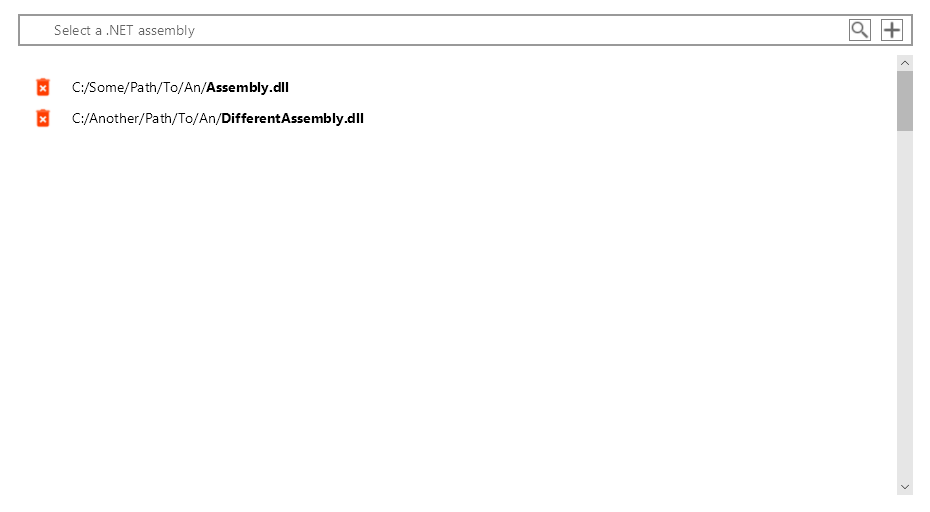
\includegraphics[width=\linewidth]{img/mockMember provider.png}
    \label{fig:pluginMember}
    \caption{Assembly configuration step}
\end{figure}

\begin{enumerate}
    \item Text field for manually entering the assembly or executable for processing
    \item Button for browsing the system for the desired assemblies of executables for processing
    \item Button for adding the manually entered path
    \item Button for revalidating the provided file paths for their existence and system permissions (not implemented, disabled)
    \item Button for removing the added file path
    \item The added file path with the file highlighted in bold
\end{enumerate}

\subsection{Documentation provider}

The documentation provider step displays the automatically discovered documentation files, alongside those that are missing. Unfortunately, this configuration step does not allow ignoring, or manually specifying documentation file paths, because of limited development time.

\subsubsection{Mock}

\begin{figure}[H]
    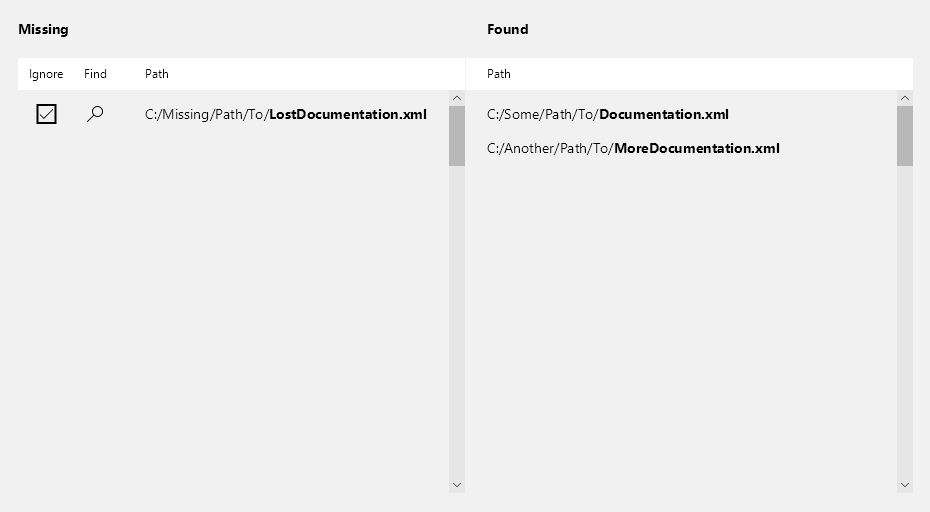
\includegraphics[width=\linewidth]{img/mockDocumentation provider.png}
    \label{fig:pluginDocumentation}
    \caption{Documentation configuration step}
\end{figure}

\begin{enumerate}
    \item Table with a list of missing documentation files
    \item Table with a list of located documentation files
\end{enumerate}

\subsection{Linker}

The linker step displays configuration options that target specific \ref{gloss:git} platforms. The user can generate documentation either for GitHub or GitLab. The choice affects the generated link format, which is platform-specific.

Next, they can decide whether the documentation will be hosted in the repository alongside the source code, or the Wiki pages. This option is necessary for GitHub, since its Wiki limits its users to a flat file structure, whereas GitLab allows structuring documentation into folder in their Wiki. Moreover, GitHub does not allow uploading multiple pages to the Wiki in bulk. Thus, if there is a lot of documentation, a user would most likely need to use the option for hosting documentation alongside the source code.

Finally, it is possible to explicitly choose whether the documentation is generated flat, or structured into individual folders. This option is relevant for GitLab, as it allows both.

\subsubsection{Mock}

\begin{figure}[H]
    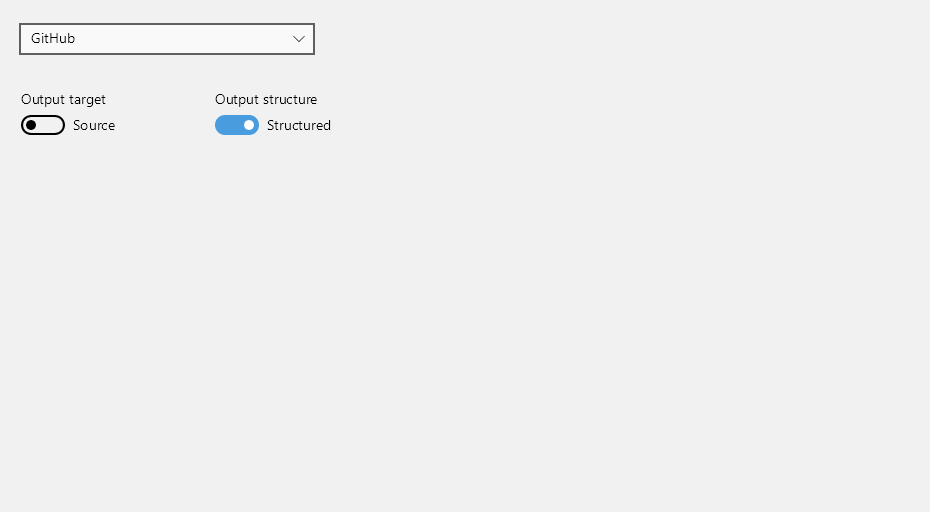
\includegraphics[width=\linewidth]{img/mockLink provider.png}
    \label{fig:pluginLinker}
    \caption{Linker configuration step}
\end{figure}

\begin{enumerate}
    \item Selection of the target \ref{gloss:git} system
    \item Toggle for linking generated documentation to source files (not implemented, disabled)
    \item Toggle for determining whether the generated output will be stored with the source code, or the Wiki
    \item Toggle for determining whether the generated output will be structured into multiple subfolders, or flat
\end{enumerate}

\subsection{Global configuration}

The global configuration affects all components, as it provides a filter for excluding specific namespaces and types from being processed. Additionally, it allows users to specify the output folder for the generated documentation.

\subsubsection{Mock}

\begin{figure}[H]
    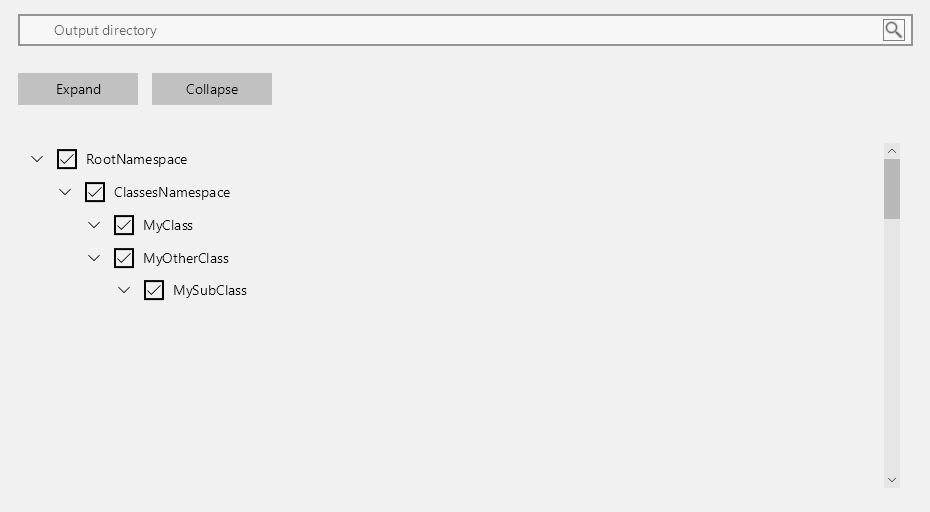
\includegraphics[width=\linewidth]{img/mockGlobal settings.png}
    \label{fig:pluginGlobal}
    \caption{Global configuration step}
\end{figure}

\begin{enumerate}
    \item Output path for the generated documentation
    \item Button for browsing the output path
    \item Buttons for toggling the expansion and collapsing of the namespace and type tree
    \item The namespace and type tree for toggling what entries are to be removed from the processing
\end{enumerate}
\chapter{Markdown for Git plugin}

This milestone covers the development of the \ref{gloss:markdown} for \ref{gloss:git} plugin described in stage \ref{num:stage10} of the \Nameref{sec:developmentStages}.

\section{Plugin structure}

The \ref{gloss:markdown} for \ref{gloss:git} plugin will be composed of components developed in \Nameref{chap:processingLibraries}.

\begin{figure}[H]
    \centering
    \label{fig:pluginStructure}
    \tikzset{every picture/.style={line width=0.75pt}} %set default line width to 0.75pt

        \begin{tikzpicture}[x=0.75pt,y=0.75pt,yscale=-1,xscale=1]
        %uncomment if require: \path (0,428); %set diagram left start at 0, and has height of 428

        %Shape: Folded Corner [id:dp38453805550218356]
        \draw   (128,110) -- (14,110) -- (14,150) -- (140,150) -- (140,122) -- cycle -- (128,110) ; \draw   (140,122) -- (130.4,119.6) -- (128,110) ;

        %Shape: Cube [id:dp9514351083967096]
        \draw   (461,30.21) -- (471.21,20) -- (590,20) -- (590,247.79) -- (579.79,258) -- (461,258) -- cycle ; \draw   (590,20) -- (579.79,30.21) -- (461,30.21) ; \draw   (579.79,30.21) -- (579.79,258) ;
        %Shape: Rectangle [id:dp28951515389797833]
        \draw   (470,68) -- (571,68) -- (571,127) -- (470,127) -- cycle ;

        %Shape: Rectangle [id:dp811482931901953]
        \draw   (470,208) -- (571,208) -- (571,241) -- (470,241) -- cycle ;

        %Shape: Rectangle [id:dp5590157968822316]
        \draw   (470,139) -- (571,139) -- (571,198) -- (470,198) -- cycle ;


        %Shape: Rectangle [id:dp0837615901192712]
        \draw   (200,10) -- (360,10) -- (360,50) -- (200,50) -- cycle ;

        %Shape: Rectangle [id:dp21181013544630467]
        \draw   (190,220) -- (390,220) -- (390,260) -- (190,260) -- cycle ;

        %Curve Lines [id:da5699658849973097]
        \draw    (70,110) .. controls (70,31.86) and (161.2,28.74) .. (198.34,29.94) ;
        \draw [shift={(200,30)}, rotate = 182.12] [color={rgb, 255:red, 0; green, 0; blue, 0 }  ][line width=0.75]    (10.93,-3.29) .. controls (6.95,-1.4) and (3.31,-0.3) .. (0,0) .. controls (3.31,0.3) and (6.95,1.4) .. (10.93,3.29)   ;
        %Curve Lines [id:da0934002278421866]
        \draw    (70,150) .. controls (70,240.75) and (140.57,238.72) .. (188.55,239.96) ;
        \draw [shift={(190,240)}, rotate = 181.59] [color={rgb, 255:red, 0; green, 0; blue, 0 }  ][line width=0.75]    (10.93,-3.29) .. controls (6.95,-1.4) and (3.31,-0.3) .. (0,0) .. controls (3.31,0.3) and (6.95,1.4) .. (10.93,3.29)   ;
        %Curve Lines [id:da9139301607505403]
        \draw    (280,50) .. controls (281.98,104.12) and (393.73,113.48) .. (458.07,110.11) ;
        \draw [shift={(460,110)}, rotate = 176.72] [color={rgb, 255:red, 0; green, 0; blue, 0 }  ][line width=0.75]    (10.93,-3.29) .. controls (6.95,-1.4) and (3.31,-0.3) .. (0,0) .. controls (3.31,0.3) and (6.95,1.4) .. (10.93,3.29)   ;
        %Curve Lines [id:da360087403261089]
        \draw    (290,220) .. controls (290,198.67) and (294,151.67) .. (460,160) ;
        \draw [shift={(460,160)}, rotate = 182.87] [color={rgb, 255:red, 0; green, 0; blue, 0 }  ][line width=0.75]    (10.93,-3.29) .. controls (6.95,-1.4) and (3.31,-0.3) .. (0,0) .. controls (3.31,0.3) and (6.95,1.4) .. (10.93,3.29)   ;
        %Shape: Rectangle [id:dp5335135464926624]
        \draw   (240,310) -- (330,310) -- (330,350) -- (240,350) -- cycle ;

        %Curve Lines [id:da34448081447371903]
        \draw    (520,260) .. controls (520,338.61) and (403.18,329.1) .. (331.08,329.99) ;
        \draw [shift={(330,330)}, rotate = 359.2] [color={rgb, 255:red, 0; green, 0; blue, 0 }  ][line width=0.75]    (10.93,-3.29) .. controls (6.95,-1.4) and (3.31,-0.3) .. (0,0) .. controls (3.31,0.3) and (6.95,1.4) .. (10.93,3.29)   ;
        %Shape: Folded Corner [id:dp9495985347442353]
        \draw   (128,310) -- (14,310) -- (14,350) -- (140,350) -- (140,322) -- cycle -- (128,310) ; \draw   (140,322) -- (130.4,319.6) -- (128,310) ;
        %Straight Lines [id:da8650986253114432]
        \draw    (240,330) -- (142,330) ;
        \draw [shift={(140,330)}, rotate = 360] [color={rgb, 255:red, 0; green, 0; blue, 0 }  ][line width=0.75]    (10.93,-3.29) .. controls (6.95,-1.4) and (3.31,-0.3) .. (0,0) .. controls (3.31,0.3) and (6.95,1.4) .. (10.93,3.29)   ;

        % Text Node
        \draw (37.11,122) node [anchor=north west][inner sep=0.75pt]   [align=left] {Input folder};
        % Text Node
        \draw (485,79) node [anchor=north west][inner sep=0.75pt]   [align=left] {\begin{minipage}[lt]{48.65pt}\setlength\topsep{0pt}
        \begin{center}
        Element\\Provider
        \end{center}

        \end{minipage}};
        % Text Node
        \draw (499,205) node [anchor=north west][inner sep=0.75pt]   [align=left] {\begin{minipage}[lt]{30.51pt}\setlength\topsep{0pt}
        \begin{center}
        Linker
        \end{center}

        \end{minipage}};
        % Text Node
        \draw (485,150) node [anchor=north west][inner sep=0.75pt]   [align=left] {\begin{minipage}[lt]{48.65pt}\setlength\topsep{0pt}
        \begin{center}
        Diagram\\Generator
        \end{center}

        \end{minipage}};
        % Text Node
        \draw (488,40) node [anchor=north west][inner sep=0.75pt]   [align=left] {Composer};
        % Text Node
        \draw (211,22) node [anchor=north west][inner sep=0.75pt]   [align=left] {Member provider};
        % Text Node
        \draw (201,231) node [anchor=north west][inner sep=0.75pt]   [align=left] {Documentation provider};
        % Text Node
        \draw (101,62) node [anchor=north west][inner sep=0.75pt]   [align=left] {*.dll, *.exe};
        % Text Node
        \draw (111,201) node [anchor=north west][inner sep=0.75pt]   [align=left] {*.xml};
        % Text Node
        \draw (351,81) node [anchor=north west][inner sep=0.75pt]   [align=left] {Types};
        % Text Node
        \draw (336,181) node [anchor=north west][inner sep=0.75pt]   [align=left] {Documentation};
        % Text Node
        \draw (261,321) node [anchor=north west][inner sep=0.75pt]   [align=left] {Printer};
        % Text Node
        \draw (394,301) node [anchor=north west][inner sep=0.75pt]   [align=left] {Elements};
        % Text Node
        \draw (31,322) node [anchor=north west][inner sep=0.75pt]   [align=left] {Output folder};
        % Text Node
        \draw (164,301) node [anchor=north west][inner sep=0.75pt]   [align=left] {Result};
    \end{tikzpicture}
    \caption{Plugin components structure}
\end{figure}

Figure \ref{fig:pluginStructure} depicts relations between each component, the input folder, and the output folder. The member and documentation providers operate in parallel, and supply necessary data to the composer component by processing files from the input folder.
The composer component depends on the element provider, linker, and diagram generator for composing the extracted data into a structured documentation.
Finally, the structured documentation is fed into the printer component, which simply generated the physical files into the designated output folder.

\section{Plugin configuration steps}

The plugin must provide configuration steps for the user to set how each component should operate. It is not necessary for the plugin to provide configuration steps for every component, as some might not be configurable. Additionally, the plugin might provide configurations that affect more than one component.

In the case of the \ref{gloss:markdown} for \ref{gloss:git} plugin, the following configuration steps are necessary in this order specifically:
\begin{itemize}
    \item Member provider
    \item Documentation provider
    \item Linker
    \item Global configuration
\end{itemize}

\subsection{Member provider}

The member provider configuration would be labeled to the user as the \textbf{Assembly} processing component, because the they would select the desired assemblies and executable \ref{gloss:dotnetlabel} files for processing.

The user can move to the next step once at least one file is provided.

\subsubsection{Mock}

\begin{figure}[H]
    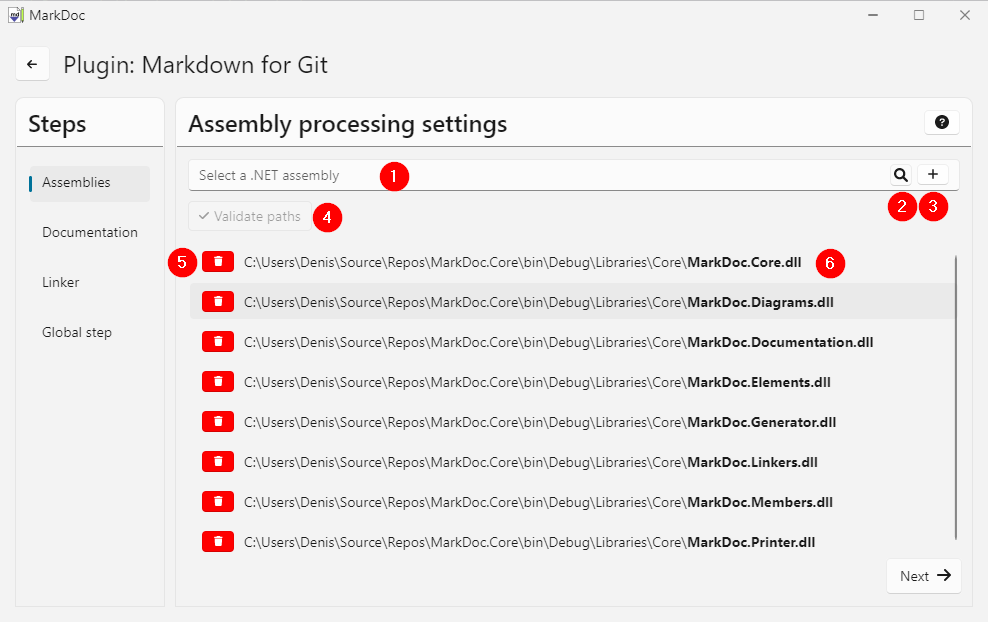
\includegraphics[width=\linewidth]{img/pluginMember.png}
    \label{fig:pluginMember}
    \caption{Assembly configuration step}
\end{figure}

\begin{enumerate}
    \item Text field for manually entering the assembly or executable for processing
    \item Button for browsing the system for the desired assemblies of executables for processing
    \item Button for adding the manually entered path
    \item Button for revalidating the provided file paths for their existence and system permissions (not implemented, disabled)
    \item Button for removing the added file path
    \item The added file path with the file highlighted in bold
\end{enumerate}

\subsection{Documentation provider}

The documentation provider step displays the automatically discovered documentation files, alongside those that are missing. Unfortunately, this configuration step does not allow ignoring, or manually specifying documentation file paths, because of limited development time.

\subsubsection{Mock}

\begin{figure}[H]
    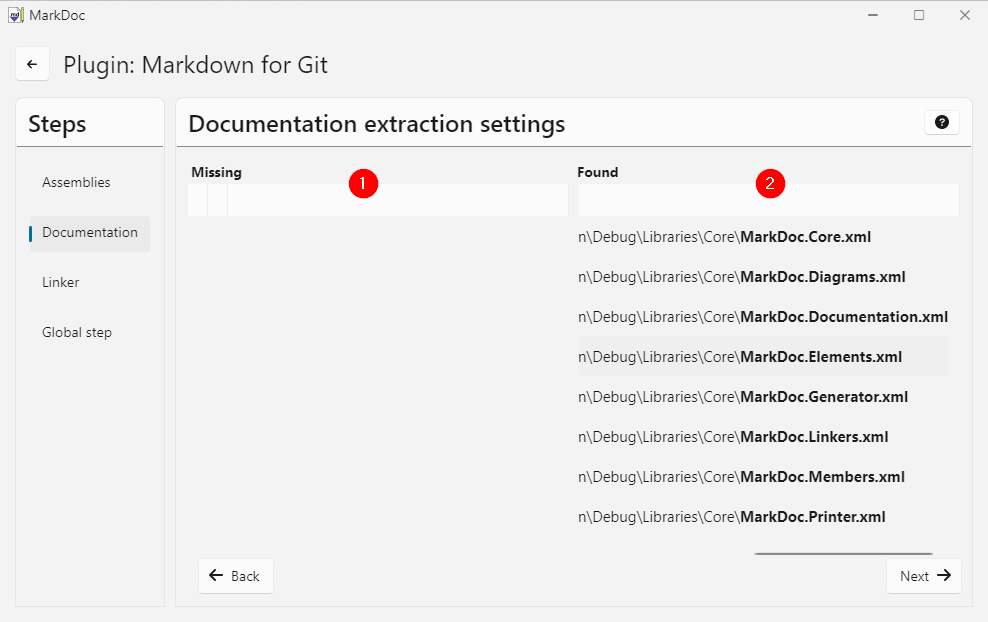
\includegraphics[width=\linewidth]{img/pluginDocumentation.png}
    \label{fig:pluginDocumentation}
    \caption{Documentation configuration step}
\end{figure}

\begin{enumerate}
    \item Table with a list of missing documentation files
    \item Table with a list of located documentation files
\end{enumerate}

\subsection{Linker}

The linker step displays configuration options that target specific \ref{gloss:git} platforms. The user can generate documentation either for GitHub or GitLab. The choice affects the generated link format, which is platform-specific.

Next, they can decide whether the documentation will be hosted in the repository alongside the source code, or the Wiki pages. This option is necessary for GitHub, since its Wiki limits its users to a flat file structure, whereas GitLab allows structuring documentation into folder in their Wiki. Moreover, GitHub does not allow uploading multiple pages to the Wiki in bulk. Thus, if there is a lot of documentation, a user would most likely need to use the option for hosting documentation alongside the source code.

Finally, it is possible to explicitly choose whether the documentation is generated flat, or structured into individual folders. This option is relevant for GitLab, as it allows both.

\subsubsection{Mock}

\begin{figure}[H]
    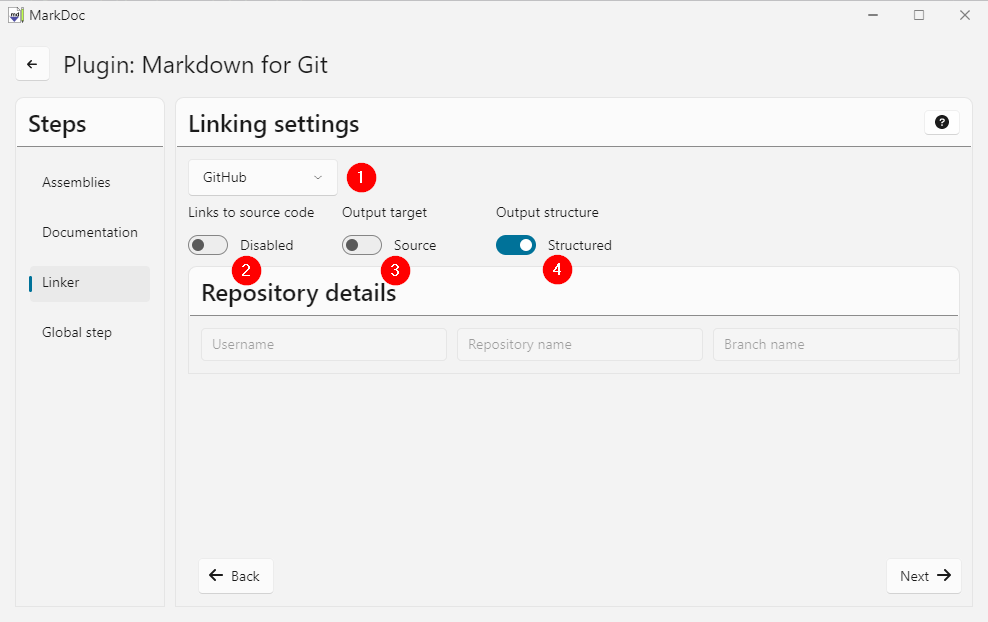
\includegraphics[width=\linewidth]{img/pluginLinker.png}
    \label{fig:pluginLinker}
    \caption{Linker configuration step}
\end{figure}

\begin{enumerate}
    \item Selection of the target \ref{gloss:git} system
    \item Toggle for linking generated documentation to source files (not implemented, disabled)
    \item Toggle for determining whether the generated output will be stored with the source code, or the Wiki
    \item Toggle for determining whether the generated output will be structured into multiple subfolders, or flat
\end{enumerate}

\subsection{Global configuration}

The global configuration affects all components, as it provides a filter for excluding specific namespaces and types from being processed. Additionally, it allows users to specify the output folder for the generated documentation.

\subsubsection{Mock}

\begin{figure}[H]
    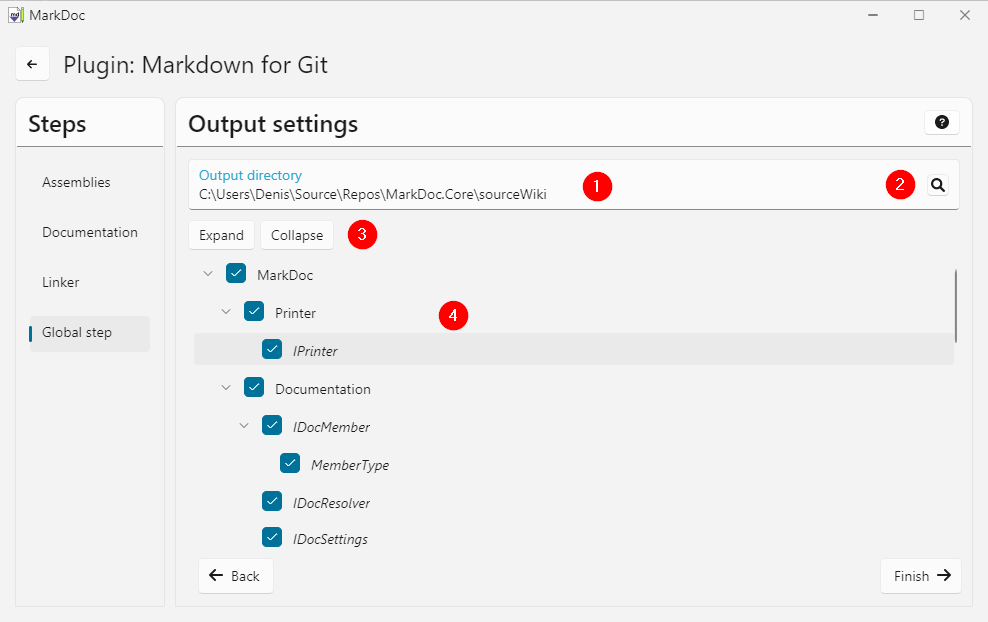
\includegraphics[width=\linewidth]{img/pluginGlobal.png}
    \label{fig:pluginGlobal}
    \caption{Global configuration step}
\end{figure}

\begin{enumerate}
    \item Output path for the generated documentation
    \item Button for browsing the output path
    \item Buttons for toggling the expansion and collapsing of the namespace and type tree
    \item The namespace and type tree for toggling what entries are to be removed from the processing
\end{enumerate}
\chapter{Performance}

One of the goals of this thesis was to ensure that the resulting application performance is comparable, if not better, to existing tools. Thus, it is necessary to evaluate whether this requirement is satisfied.

The thesis project source code would be used for benchmarking performance.
Specifically, projects containing the shared interfaces shall be used as the source of processing\footnote{Located in the solution folder, \textit{Libraries/Core/}. Everything except the \textit{Constants} project.}.
The tests will run on a Windows Operating System, and shall compare performance of the project to DocFX, and Doxygen. Source browser was excluded due to unclear instructions and inability to make it work using existing examples. Other solutions were also excluded as they do not produce proper documentation.

Testing will measure elapsed time for generating the documentation. This will be done by running each tool via Windows PowerShell using the \textit{Measure-Command}. If the resulting tool is consistently perceived to be considerably slower than existing tools, then the performance requirement can be deemed as unsatisfied.

\section{Configurations}

\subsection{Custom}

The custom tool represents the project developed in the context of this thesis.
The performed benchmarking is relevant for the \ref{gloss:markdown} for \ref{gloss:git} plugin, as it is currently the only available plugin for the tool.
For consistency, a console-based application\footnote{The console can be found in the repository as \textit{MarkDoc.CLI}} was created that loads the defined configuration and simply executes it.
The console application is missing crucial features such as argument validation, error handling, etc.; thus, it primarily serves for testing purposes.

\subsection{Doxygen}

Configuring Doxygen was a simple and intuitive process, making it a worthy contender. The tool was configured to:
\begin{itemize}
    \item Document all entities, and not exclude those without documentation
    \item Optimize results for Java or C\# output
    \item Generate plain \ref{itm:html} output with search capabilities
    \item Use the built-in class diagram generator
\end{itemize}

Version \textit{1.9.5} was used for testing.

\subsection{DocFX}

Configuring DocFX was not an intuitive process, as everything is done via the \ref{itm:cli}. However, the documentation was sufficient for configuring the tool to process only the desired input.

Version \textit{2.59.4} was used for testing.

\section{Results}

\begin{table}[H]
    \caption{Documentation generating tools performance comparison}
    \centering
    \label{tab:toolPerformance}
    \begin{tabular}{lrrr}
    \hline
    \textbf{Run}            & \multicolumn{1}{l}{\textbf{Custom}}    & \multicolumn{1}{l}{\textbf{Doxygen}}    & \multicolumn{1}{l}{\textbf{DocFX}}       \\ \hline
    \multicolumn{1}{|l|}{1} & \multicolumn{1}{r|}{864 ms}            & \multicolumn{1}{r|}{3609 ms}            & \multicolumn{1}{r|}{34268 ms}            \\ \hline
    \multicolumn{1}{|l|}{2} & \multicolumn{1}{r|}{968 ms}            & \multicolumn{1}{r|}{1784 ms}            & \multicolumn{1}{r|}{28662 ms}            \\ \hline
    \multicolumn{1}{|l|}{3} & \multicolumn{1}{r|}{869 ms}            & \multicolumn{1}{r|}{1664 ms}            & \multicolumn{1}{r|}{28681 ms}            \\ \hline
    \multicolumn{1}{|l|}{4} & \multicolumn{1}{r|}{846 ms}            & \multicolumn{1}{r|}{1660 ms}            & \multicolumn{1}{r|}{28681 ms}            \\ \hline
    \textbf{Average}        & \multicolumn{1}{l}{\textit{886.75 ms}} & \multicolumn{1}{l}{\textit{2179.25 ms}} & \multicolumn{1}{l}{\textit{30022.25 ms}} \\ \hline
    \end{tabular}
\end{table}

As clearly shown, the custom tool is at least ten times faster than Doxygen, and a hundred times faster than DocFX. This is most likely because the custom tool is specifically designed for \ref{gloss:dotnetlabel} projects, whereas the other two are polyglots that support different languages and project types. Additionally, the custom tool was designed with performance in mind, and utilizes caching techniques, lazy loading, and, most importantly, generates documentation via reflection.
% \include{...}
% \include{...}
\chapter*{Summary}
\addcontentsline{toc}{chapter}{Summary}

The defined goal of this thesis was reached successfully by producing a working custom documentation-generating tool for \ref{gloss:dotnetlabel} libraries.

\section*{Goal fulfillment}
\addcontentsline{toc}{section}{Goals and their fulfillment}

This thesis aimed to create a custom documentation-generating tool for \ref{gloss:dotnetlabel} projects using appropriate design patterns \cite{humblot_design_2021} and to satisfy user needs for extensibility, ease of use, modern design, support for many output formats, and comparable performance to existing tools.

The resulting project is:
\begin{itemize}
    \item A set of abstract interfaces defining key parts of the whole application.
    \item A set of concrete components that are independent of each other.
    \item A plugin composed of the developed components for generating \ref{gloss:markdown} documentation.
    \item A \ref{itm:gui} application for hosting plugins and allowing users to configure and execute them.
\end{itemize}

The decoupled architecture provides maximum extensibility - if a user is missing a feature, they can always add it. The \ref{itm:ui}/\ref{itm:ux} of the tool is simple, with hints and labels, making it easy to use. Thanks to the extensibility, the tools supports endless output formats; however, the resulting project so far supports \ref{gloss:markdown} only. Moreover, the tool is very performant and can compete with industry standards such as Doxygen.

Given these facts, the goal of this thesis is fulfilled.

\section*{Open-source} \label{sec:openSource}
\addcontentsline{toc}{section}{Open-source}

The source code for ModularDoc can be found on GitHub, as well as the source for this thesis, as it was written using \LaTeX:
\begin{description}
    \item[Project:] \textit{\nolinkurl{https://github.com/hailstorm75/ModularDoc}}
    \item[Thesis:] \textit{\nolinkurl{https://github.com/hailstorm75/ModularDoc.Thesis}}
\end{description}

\section*{Personal achievements}
\addcontentsline{toc}{section}{Personal achievements}

Reaching this state of the project is an achievement to be proud of. Considerable effort was put into retaining proper modularity and decoupling business logic from specific frameworks and platforms. In addition, a broader understanding of documentation and the C\# language was gained, alongside experience with solving complex problems without the assistance of documentation or help from fellow developers.

One documented personal goal was to write some of the libraries in F\#. The choice to deviate from C\# had minor benefits. The produced code is complicated to maintain, specifically in the composer component. The reasons for such a damaging outcome are caused by lack of proper functional programming experience and limited capabilities of core F\# features.

ModularDoc source code has flaws, as any software; however, this tool can provide actual value to its users in its current state. And that is an indicator of success.

\section*{Future plans}
\addcontentsline{toc}{section}{Future plans}

Completing the initial goal was only the beginning. The project needs a suite of tests validating the code's behavior to gain user trust. Furthermore, to gain collaborator interest, the project needs a well-written wiki on how to extend ModularDoc.

By themselves, said tasks are no less complex than creating the tool itself, as both require great care and attention to guarantee positive results. Even if the project does not get the desired awareness from the open-source collaborator community, completing said tasks will still provide valuable experience.


%%% Bibliography
\include{literatura}

%%% Attachments to thesis, if any. Each attachment must be referenced at
%%% least once in your own text. The appendices are numbered.
% \part*{\Prilohy}
% \appendix
% \section*{Appendix: ModularDoc compiled} \label{app:modularDocCompiled}
\addcontentsline{toc}{section}{ModularDoc compiled}

Compiled source code (see \Nameref{app:modularDocSourceCode}) of the resulting application of this thesis - ModularDoc.

Prerequisites and instructions for running the compiled application are provided in \Nameref{sec:userGuide}.
% \section*{Appendix: ModularDoc source code} \label{app:modularDocSourceCode}
\addcontentsline{toc}{section}{ModularDoc source code}

Source code of the resulting application of this thesis - ModularDoc.
It is written in C\# and F\# on the \ref{gloss:dotnetlabel} 6 platform.

The provided source is a snapshot of its version-controlled state hosted on GitHub.
The state was captured on the 11th of December, 2022, and corresponds to the following \ref{gloss:git} commit identifier: \textit{00e585f881e92ebf6c6d7e4da24ca763b7671e3e}.

Instructions for modifying the source code, alongside instructions on how to get its latest version-controlled state, are provided in \Nameref{subsec:accessingSourceCode}.

% \include{...}
% \include{...}

\end{document}
